
\chapter{Elementare Zahlentheorie}




\section*{Lernziele}
Sie kennen die
\begin{itemize}
\item Grundlagen der Teilbarkeitslehre.
\item den Begriff der Primzahl.
\item das kgV und den ggT und wie diese mithilfe des  euklidischen Algorithmus berechnet werden.
\item das Lemma von Bézout.
\item den chinesischen Restsatz.
\item den kleinen Fermatschen Satz.
\end{itemize}
Sie verstehen
\begin{itemize}
\item wieso und wie ganze Zahlen in ihre Primfaktoren zerlegt werden können.
\item die modulare Arithmetik.
\item den Zusammenhang vom chinesischen Restsatz und der Lösbarkeit von simultanen Kongruenzen.
\end{itemize}
Sie sind in der Lage
\begin{itemize}
\item die Stellenwertsysteme ineinander umzurechnen.
\item Systeme simultaner Kongruenzen aufzulösen.
\end{itemize}


\section*{Literatur und Links}
\begin{itemize}
\item Euklidischer Algorithmus:\\
\url{http://de.wikipedia.org/wiki/Euklidischer_Algorithmus}\\
\end{itemize}


Analog zu unserem Vorgehen mit den natürlichen Zahlen wollen wir auch die \textit{ganzen Zahlen} informell einführen. Wir definieren
\[
\Z:= \{..,-2,-1,0,1,2,...\}.
\]
Die Motivation die Menge $\N$ zur Menge $\Z$ erweitern zu wollen fusst auf der Tatsache, dass für feste natürliche Zahlen $k,k'$ im Allgemeinen die Gleichung
\[
 k+x=k'
\]
keine Lösung in $\N$ besitzt. Es ist in der Tat so, dass bei der Konstruktion von $\Z$ aus $\N$ (was wir nicht tun werden) die Menge $\Z$ im Prinzip als die Menge aller Lösungen von solchen Gleichungen eingeführt wird.

Wir wollen es als gegeben erachten, dass die Multiplikation und die Addition derart von $\N$ auf $\Z$ fortgesetzt werden können, dass folgende Rechenregeln bestehen:

\begin{rk}[Rechenregeln auf $\Z$]
Für alle $r,s,z\in\Z$ gelten folgende Gleichungen.
\begin{align*}
-1\cdot z&=-z\\
-(-z)&=z\\
-z+z&=0 &\text{ Inverse Elemente bezüglich }+\\
0\cdot z&=0 &\text{ Absorbtion}\\
1\cdot z&=z &\text{ Neutrales Element bezüglich }\cdot\\
0+z&=z &\text{ Neutrales Element bezüglich }+\\
r(sz)&=(rs)z &\text{ Assoziativität von } \cdot\\
r+(s+z)&=(r+s)+z &\text{ Assoziativität von }+\\
rs&=sr &\text{ Kommutativität von }\cdot\\
r+s&=s+r &\text{ Kommutativität von }+\\
r(s+z)&=rs+rz &\text{ Distributivität}\\
rx=ry&\Rightarrow x=y\lor r=0&\text{Kürzbarkeit}
\end{align*}
\end{rk}

\begin{df}
 Wir definieren die \textit{Subtraktion}
\[
 -:\Z\times\Z\rightarrow\Z
\]
durch
\[
 x-y:=x+(-y),
\]
die \textit{Betragsfunktion}
\[
 |\cdot|:\Z\rightarrow\N
\]
durch
\[
 |z|=\begin{cases}
      z&\text{falls } z\in\N\\
      -1\cdot z&\text{sonst}
     \end{cases}
\]
und die Relation $\leq$ durch
\[
x\leq y:\Leftrightarrow\,\exists n\in\N\,(x+n=y).
\]
\end{df}



\section{Teilbarkeit und Euklidischer Algorithmus}
\begin{df}
 Sind $x,y\in\mathbb{Z}$ ganze Zahlen, so sagen wir, dass $x$ \textit{ein Teiler von} $y$ ist, falls es ein $k\in\mathbb{Z}$ gibt mit $xk=y$. Wir schreiben in diesem Fall $x|y$. Es gilt also
\[
 x|y:\Leftrightarrow \exists k\in\Z(y=xk).
\]
Mit $T(y)$ bezeichnen wir die Menge aller natürlichen Zahlen, welche Teiler von $y$ sind, also $T(y)=\{x\in\N\mid x|y\}$.
\end{df}
\begin{bsp}~
 \begin{enumerate}
  \item Die Zahl $1$ ist ein Teiler jeder ganzen Zahl $z$, da $1\cdot z=z$.
\item $T(0)=\N$.
 \end{enumerate}

\end{bsp}
\begin{rk}
 Die Teilbarkeitsrelation ist reflexiv und transitiv auf der Menge $\Z$, auf der Menge $\N$ ist die Teilbarkeitsrelation sogar eine Halbordnung (wieso nicht auf der Menge $\Z$?).
\end{rk}
\begin{proof}
Wir zeigen, dass die Teilbarkeitsrelation reflexiv, transitiv und für natürliche Zahlen auch antisymmetrisch ist.
\begin{itemize}
\item Reflexivität: Dies gilt, da jede ganze Zahl sich selbst teilt.
\item Transitivität: Seien $x,y,z$ ganze Zahlen. Aus $x|y$ und $y|z$ folgt, dass es ganze Zahlen $k_1,k_2$ gibt mit $x\cdot k_1=y$ und $y\cdot k_2=z$. Es folgt
\[
x\cdot(k_1\cdot k_2)=(x\cdot k_1)\cdot k_2=y\cdot k_2=z.
\]
 Somit existiert eine ganze Zahl $k$ (nämlich $k=k_1\cdot k_2$) mit $k\cdot x=z$, also gilt $x|z$ wie gewünscht.\qedhere
\item Antisymmetrie auf $\N$: Wir müssen zeigen, dass für natürliche Zahlen $x$ und $y$ aus $x|y$ und $y|x$ folgt, dass $x=y$ gilt. Es gelte also $xk=y$ und $x=yr$ für ganze Zahlen $k,r$. Es folgt
\[
x=yr=(xk)r=x(kr)
\]
und $kr=1$. Daraus ergeben sich zwei mögliche Fälle; $k=r=1$ oder $k=r=-1$. Im Fall $k=r=-1$ folgt $x=-y$, was im Widerspruch dazu steht, dass $x$ und $y$ natürliche Zahlen sind. Es bleibt also nur der Fall $k=r=1$ und somit, wie gewünscht, $x=y$.
\end{itemize}
\end{proof}

\begin{bsp}
Das Hasse-Diagramm der Teilbarkeitsrelation auf der Menge $T(30)$:
\begin{center}
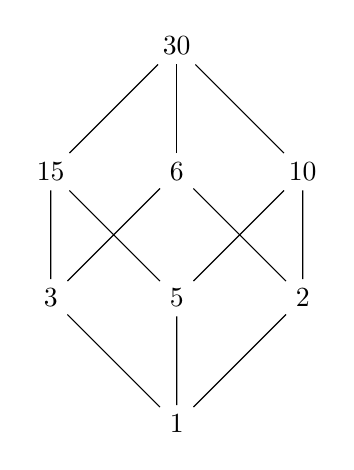
\begin{tikzpicture}[scale=0.8]
  \node (1) at (0,0) {$1$};
  \node (2) at (2,2) {$2$};
  \node (3) at (-2,2) {$3$};
  \node (5) at (0,2) {$5$};
  \node (15) at (-2,4) {$15$};
  \node (6) at (0,4) {$6$};
  \node (10) at (2,4) {$10$};
  \node (30) at (0,6) {$30$};
  \draw (1) -- (3) -- (15) -- (30) -- (10) -- (2)--(1)--(5)--(15)--(3)--(6)--(2);
  \draw (5) -- (10);
  \draw (6) -- (30);
\end{tikzpicture}
\end{center}
Das Hasse-Diagramm der Teilbarkeitsrelation auf der Menge $T(90)$:
\begin{center}
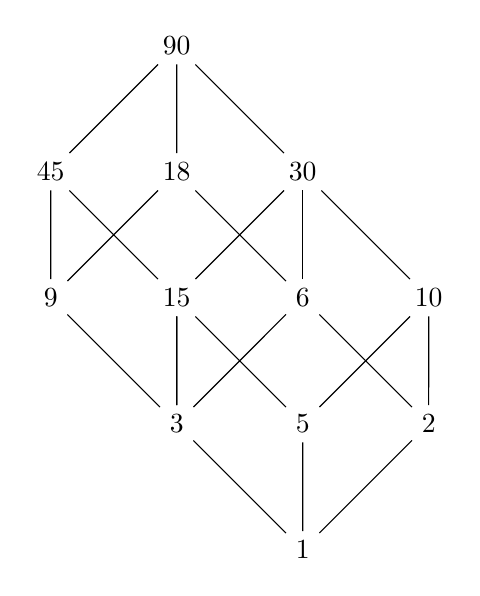
\begin{tikzpicture}[scale=0.8]
  \node (1) at (0,0) {$1$};
  \node (2) at (2,2) {$2$};
  \node (3) at (-2,2) {$3$};
  \node (5) at (0,2) {$5$};
  \node (15) at (-2,4) {$15$};
  \node (6) at (0,4) {$6$};
  \node (10) at (2,4) {$10$};
  \node (30) at (0,6) {$30$};
  \node (45) at (-4,6) {$45$};
  \node (18) at (-2,6) {$18$};
  \node (9) at (-4,4) {$9$};
  \node (90) at (-2,8) {$90$};
  \draw (1) -- (3) -- (15) -- (30) -- (10) -- (2)--(1)--(5)--(15)--(3)--(6)--(2);
  \draw (5) -- (10);
  \draw (6) -- (18)--(9)--(3)--(15)--(45)--(90)--(30);
  \draw (6) -- (30);
  \draw (9) -- (45);
  \draw (18) -- (90);
\end{tikzpicture}
\end{center}
\end{bsp}

\begin{rk}\label{Zeinheiten}
Sind $x,y\in\Z$ und gilt $x\cdot y=1$ so gilt $|x|=|y|=1$.
\end{rk}


\begin{satz}[Teilen mit Rest]
 Sind $n,m\in\N\backslash\{0\}$, dann gibt es eindeutig bestimmte Zahlen $k,r\in\N$, so dass Folgendes gilt:
\begin{enumerate}
\item $m=kn+r$
 \item $r<n$
\end{enumerate}
Wir sagen in diesem Zusammenhang, dass die Zahl $r$ den \textit{Rest} von der (ganzzahligen) Division von $m$ durch $n$ ist.
\end{satz}
\begin{proof}
 Seien $n,m\in\N\backslash\{0\}$ beliebig. Die Menge
\[
 M:=\{k\in\N\mid kn\leq m\}
\]
ist endlich (da $n\geq 1$), somit gibt es ein maximales Element $k_0\in M$. Wir definieren $r:=m-k_0n$. Da $k_0\in M$ gilt, ist $r\in\N$. Es gilt
\[
 k_0n+r=k_0n+(m-k_0n)=m.
\]
Falls $r\geq n$ wäre, dann würde
\[
 m-(k_0+1)n=m-(k_0n+n)=r-n\geq 0
\]
und somit $k_0+1\in M$ gelten, was im Widerspruch zur Maximalität von $k_0$ in $M$ steht. Wir müssen nun noch die Eindeutigkeit zeigen. Es genügt zu zeigen, dass für $r,r'<n$
\[
 (kn+r=k'n+r')\Rightarrow (k=k')
\]
gilt. Wir machen einen Beweis durch Widerspruch und nehmen also $k\neq k'$ an. Aus Symmetriegründen können wir $k<k'$ und somit $k'=k+p$ mit $p>0$ annehmen. Es gilt also
\begin{align*}
 kn+r=k'n+r'=(k+p)n+r'=kn+pn+r'
\end{align*}
und somit
\[
 r=pn+r'\geq n,
\]
ein Widerspruch.
\end{proof}

\begin{ueb}
	Schreiben Sie in der Programmiersprache Ihrer Wahl eine Funktion, die zwei positive ganze Zahlen mit Rest teilt (natürlich ohne die Verwendung des Modulo Operators).
\end{ueb}
\begin{lsg}
	\ifthenelse{\boolean{ml}}{
        Vgl. Code in der Vorlesung.
		}{~
		Elektronisch zu lösen.
	}
\end{lsg}

\begin{df}
Seien $n,m\in\Z$. Wir definieren das \textit{kleinste gemeinsame Vielfache von $n$ und $m$} als
\[
 kgV(n,m):=\min\{k\in\N\mid n|k\wedge m|k\}.
\]
Ist $n\neq0$ oder $ m\neq 0$, dann definieren wir den \textit{grössten gemeinsamen Teiler} von $n$ und $m$ als
\[
 ggT(n,m):=\max\{k\in\N\mid k|n\wedge k|m\}.
\]
\end{df}

\begin{lm}\label{lm:lemmaggT}
 Sind $x,y,z\in\Z$, dann sind folgende Aussagen äquivalent:
\begin{enumerate}
\item[1.] $ x|y\wedge x|z$
\item[2.] $x|y\wedge x|(y-z) $
\end{enumerate}
\end{lm}
\begin{proof}
 $1.\Rightarrow 2.$: Wenn $x|y\wedge x|z$, dann gibt es ganze Zahlen $k,k'\in\Z$, so dass $y=kx$ und $z=k'x$. Es gilt also $y-z=kx-k'x=(k-k')x$.

$2.\Rightarrow 1.$: Es seien $k,k'\in\Z$, so dass $y=kx$ und $y-z=k'x$. Durch Einsetzen erhält man $ kx-z=k'x $ und somit $z=kx-k'x=x(k-k')$.
\end{proof}

\begin{satz}[Euklidischer Algorithmus]\label{satz:euklid}
 Für $n,m\in\N$ mit $0<n< m$ gilt
\[
 ggT(n,m)=ggT(n,m-n)=ggT(m,m-n).
\]
\end{satz}
\begin{proof}
Aus Lemma~\ref{lm:lemmaggT} folgt für $n,m\in\N$ mit $n<m$
\[
\{k\in\N\mid k|n\wedge k|m\}=\{k\in\N\mid k|n\wedge k|(m-n)\}.
\]
Daraus folgt weiter
\begin{align*}
ggT(n,m)=\max\{k\in\N\mid k|n\wedge k|m\}=\max\{k\in\N\mid k|n\wedge k|(m-n)\}=ggT(n,m-n).
\end{align*}
Die Gleichung
\[
 ggT(n,m)=ggT(m,m-n)
\]
folgt analog aus Lemma~\ref{lm:lemmaggT}.
\end{proof}

\begin{rk}[Euklidischer Algorithmus]
Aus dem eben bewiesenen Satz~\ref{satz:euklid} erhalten wir direkt einen rekursiven Algorithmus zur Berechnung des $ggT$. Beispielhaft geht man dabei wie folgt vor:
\begin{align*}
ggT(45,25)&\stackrel{Satz~\ref{satz:euklid}}{=}ggT(25,20)\\
&\stackrel{Satz~\ref{satz:euklid}}{=}ggT(20,5)\\
&\stackrel{Satz~\ref{satz:euklid}}{=}ggT(5,15)\\
&\stackrel{Satz~\ref{satz:euklid}}{=}ggT(5,10)\\
&\stackrel{Satz~\ref{satz:euklid}}{=}ggT(5,5)=5.
\end{align*}
Dieses Vorgehen lässt sich direkt in Java umsetzen:
\begin{framed}
\begin{lstlisting}[language=Java]
int ggT(int n,int m){
    if(n == m) return n;
    if(n < m) return ggT(n, m - n);
    return ggT(m, n - m);
}
\end{lstlisting}
\end{framed}
Betrachten wir nochmals den Satz~\ref{satz:euklid}, dann sehen wir, dass wir mehrere Schritte zu einem einzigen Schritt zusammenfassen können. Bei $x>y$ wird nämlich, zum Berechnen von $ggT(y,x)$ so oft $y$ von $x$ subtrahiert, bis das Resultat kleiner oder gleich $y$ ist. Man kann all diese Subtraktionen also durch eine einzige Division mit Rest ersetzen.
Die beispielhafte Berechnung von $ggT(45,25)$ können wir nun als $2$ Divisionen mit Rest darstellen:
\begin{align*}
45 &= 1 \cdot 25 + 20\\
25 &= 1 \cdot 20 + \underbrace{5}_{ggT(45,25)}.
\end{align*}
Zusammenfassend stellen wir fest, dass
\[
ggT(y,x)=ggT(y,R(x,y))
\]
mit
\[
R(x,y)=\text{ der Rest der Division von }x\text{ durch }y
\]
gilt. Die Funktion $R(x,y)$ steht in vielen Programmiersprachen als ``modulo Funktion'' zur Verfügung und wird im Quellcode oft durch das Prozentzeichen $\%$ aufgerufen. Dies eröffnet die Möglichkeit den euklidischen Algorithmus kompakter zu notieren:\\

\lstset{language=Java}
\begin{framed}
\begin{lstlisting}
int ggT(int n, int m){
    if(n == 0) return m;
    if(n < m) return ggT(m % n, n);
    return ggT(n % m, m);
}
\end{lstlisting}
\end{framed}
\end{rk}

\begin{ueb}
	Benutzen Sie den euklidischen Algorithmus um $ggT(27,96)$ auszurechnen (notieren Sie die Zwischenresultate).
\end{ueb}
\begin{lsg}
	\ifthenelse{\boolean{ml}}
		{
			\begin{align*}
				ggT(27,96) &= ggT(96 \% 27, 27)\\
				 &= ggT(15, 27) = ggT(27 \%15,15)\\
				 &=ggT(12,15)=ggT(15 \%12,12)\\
				 &=ggT(3,12)=ggT(12\%3,3)\\
				 &=ggT(0,3)=3
			\end{align*}
		}
		{~
			\answerspace{6cm}
		}
\end{lsg}
\begin{df}
 Zwei ganze Zahlen $x,y$ heissen \textit{teilerfremd}, wenn $ggT(x,y)=1$ gilt.
\end{df}

%\begin{ern}
%In den übungen haben Sie bewiesen, dass man das Prinzip der vollständigen Induktion dahingehend verallgemeinern kann, dass man in der Induktionsannahme auf alle ``Vorgängerfälle'' Bezug nehmen darf. Formal haben Sie gezeigt, für jede Menge $X\subseteq\N$ mit der Eigenschaft
%\[
%\forall n\in\N\big(\forall m<n\,(m\in X\Rightarrow n\in X)\big),
%\]
%$X=\N$ gilt. Dieses Verfahren werden wir im folgenden Beweis anwenden.
%\end{ern}

\begin{thrm}[Lemma von Bézout]\label{hauptideal}
Sind $x,y\in\Z$ mit $x,y\neq 0$, dann gibt es ganze Zahlen $a,b$ so dass
\[
 ggT(x,y)=ax+by
\]
gilt. Die Zahlen $a$ und $b$ werden Bézout Koeffizienten genannt.
\end{thrm}
\begin{proof}
	Wir können ohne Einschränkung der Allgemeinheit $x,y\geq 1$ annehmen und die Behauptung
	\begin{align*}
		\forall x,y\geq 1\;\exists a,b\in\Z\;(ggT(x,y)=ax+by).
	\end{align*}
	beweisen. Wir führen den Beweis durch Widerspruch. Es gebe also natürliche Zahlen $x,y\geq 1$ mit
	\begin{align*}
		\varphi(x,y):\Leftrightarrow \forall a,b\in\Z\;(ax+by\neq ggT(x,y)).
	\end{align*}
	Insbesondere existieren folgende kleinste natürliche Zahlen (Methode des kleinsten Verbrechers):
	\begin{align*}
		x_0&=\min \{n\geq 1 \mid \exists k\geq 1\;\varphi(n,k)\} = \min\{n\geq 1 \mid \exists k\geq 1\,\forall a,b\in\Z\;(an+bk\neq ggT(n,k))\}\\
		y_0&=\min \{n\geq 1 \mid \varphi(x_0,n)\}=\min\{n\geq 1 \mid \forall a,b\in\Z\;(ax_0+bn\neq ggT(x_0,n))\}
	\end{align*}
	Es gilt offensichtlich $x_0\neq y_0$ und $\varphi(x,y)\Leftrightarrow\varphi(y,x)$. Wir können daher ohne Einschränkung $x_0<y_0$ annehmen. Weil $1\leq y_0-x_0<y_0$ gilt, gibt es ganze Zahlen $a,b\in\Z$ mit $ax_0+b(y_0-x_0) = ggT(x_0,y_0-x_0)$. Mit dem Euklidischen Algorithmus folgt daraus der gesuchte Widerspruch (zur Wahl von $x_0$ und $y_0$):
	\begin{align*}
		(a-b)x_0+by_0 &=ax_0-bx_0+by_0\\
				      &=ax_0+b(y_0-x_0)\\
					  &= ggT(x_0,y_0-x_0)\\
					  &=ggT(x_0,y_0)
	\end{align*}



%Wir beweisen das Theorem exemplarisch für den Fall, dass $ggT(m,n)=1$ gilt. Ohne Einschränkung sei $m>n$. Sind $x,y$ beliebige ganze Zahlen, dann bezeichnen wir
%\begin{align*}
%R(x,y):=\begin{cases}
%\text{ Der Rest von der ganzzahligen Division von $x$ durch $y$}&\text{falls }x,y>0\\
%0&\text{sonst.}
%\end{cases}
%\end{align*}
%Wir definieren rekursiv eine absteigende Folge $(r_i)_{i\in\N}$ von natürlichen Zahlen wie folgt:
%\begin{align*}
%r_i=\begin{cases}
%m&\text{falls }i=0\\
%n&\text{falls }i=1\\
%R(r_{i-2},r_{i-1})&\text{sonst.}
%\end{cases}
%\end{align*}
%Da es keine echt absteigende Folge von natürlichen Zahlen gibt, muss die Folge der $(r_i)_{i\in\N}$ stationär werden. Es folgt also aus der Definition der Folge $(r_i)_{i\in\N}$, dass es ein $p\in\N$ gibt, so dass $r_{p}\neq0$ und für alle $p`>p$ gilt $r_{p`}=0$. Es sei $(\lambda_i)_{i\in\N}$ die durch $(r_i)_{i\in\N}$ eindeutig bestimmte Folge natürlicher Zahlen mit der Eigenschaft (*):
%\begin{align*}
%r_0&=\lambda_0\cdot r_1+r_2\\
%r_1&=\lambda_1\cdot r_2+r_3\\
%&\vdots\\
%r_{p-2}&=\lambda_{p-2}\cdot r_{p-1}+r_{p}
%\end{align*}
%\textbf{Behauptung}: $r_p=1$\\
%\textbf{Beweis}: Wir zeigen, dass $r_p$ ein Teiler von allen $r_i$ mit $i\leq p$ ist. Weil $r_0=m,r_1=n$ teilerfremd sind, gilt dann $r_p=1$. Wir beweisen mit (der allgemeinen Version von) Induktion für alle $k\in\N$, dass entweder $r_p|r_{p-k}$ oder $k>p$ gilt.
%Falls $k>p$ ist, dann sind wir fertig. Wir können also ohne Einschränkung der Allgemeinheit annehmen, dass $k\leq p$ gilt. Nach Induktionsannahme ist nun $r_p$ ein Teiler von $r_{p-(k-1)}$ und von $r_{p-(k-2)}$, es gibt also ganze Zahlen $x,y$ mit $x\cdot r_p=r_{p-(k-1)}$ und $y\cdot r_p=r_{p-(k-2)}$. Insgesamt haben wir dann
%\begin{align*}
%r_{p-k}=\lambda_{p-k}\cdot r_{p-k+1}+r_{p-k+2}=\lambda xr_{p}+yr_{p}=r_{p}(\lambda x+y)
%\end{align*}
%und somit wie gewünscht, dass $r_p$ ein Teiler von $r_{p-k}$ ist.\\
%Wir können nun das Gleichungssystem $(*)$ als
%\begin{align*}
%r_0&=\lambda_0\cdot r_1+r_2\\
%r_1&=\lambda_1\cdot r_2+r_3\\
%&\vdots\\
%r_{p-2}&=\lambda_{p-2}\cdot r_{p-1}+1
%\end{align*}
%schreiben. Dies ist jedoch mit
%\begin{align*}
%1&=r_{p-2}-\lambda_{p-2}r_{p-1}\\
%r_{p-1}&=r_{p-3}-\lambda_{p-3}r_{p-2}\\
%&\vdots\\
%r_{p-i}&=r_{p-i-2}-\lambda_{p-i-2}r_{p-i-1}\\
%&\vdots\\
%\underbrace{r_{p-p+2}}_{r_2}&=\underbrace{r_{p-p}}_{m}-\lambda_{0}\underbrace{r_{p-p+1}}_{n}
%\end{align*}
%äquivalent. Indem wir nun sukzessiv (von unten beginnend) in jeder Zeile des Gleichungssystems die $r_i$ auf der rechten Seite durch eine Summe von Vielfachen von $n$ und $m$ ersetzen, erhalten wir zuoberst im Gleichungssystem für geeignete $s,\delta_i,\gamma_i$ eine Gleichung von der gewünschten Gestalt
%\[
%1=\sum_{i=1}^{s}\delta_in-\gamma_im=\sum_{i=1}^{s}\delta_in-\sum_{i=1}^{s}\gamma_im=n\sum_{i=1}^{s}\delta_i-m\sum_{i=1}^{s}\gamma_i.\qedhere
%\]
\end{proof}

\begin{ueb}
	Zeigen Sie, dass Bézout Koeffizienten nicht eindeutig sind.
	\begin{lsg}
		Es sei en $a$ und $b$ Bézout Koeffizienten von $x$ und $y$. Es gilt:
		\begin{align*}
			ggT(a,b) = ax+by = ax+by+xy-xy=ax+xy+by-xy=(a+y)x+(b-x)y
		\end{align*}
	\end{lsg}
\end{ueb}


\begin{bsp}
 Wir wollen ganze Zahlen $a$ und $b$ finden, die die Gleichung
 \[
 a\cdot 504+b\cdot 29=ggT(504,29)=1
 \]
 erfüllen.
\begin{itemize}
 \item Schritt 1: Sukzessives Teilen mit Rest.
\begin{align*}
	504 &= 17 \cdot 29 + 11\\
	29 &= 2 \cdot 11 + 7\\
	11 &= 1 \cdot 7 + 4\\
	7 &= 1 \cdot 4 + 3\\
	4 &= 1 \cdot 3 + \underbrace{1}_{ggT(504,29)}.
\end{align*}
 \item Schritt 2: ``Rückwärts einsetzen''.
 \begin{align*}
	1&=4-3\\
	&=(11-7)-(7-4)\\
	&=((504-17\cdot 29)-(29-2\cdot 11))-((29-2\cdot 11)-(11-7))\\
	&=((504-17\cdot 29)-(29-2\cdot (504-17\cdot 29)))\\
	&\phantom{abst}-((29-2\cdot (504-17\cdot 29))-((504-17\cdot 29)-(29-2\cdot 11)))\\
	&=((504-17\cdot 29)-(29-2\cdot (504-17\cdot 29)))
	-((29-2\cdot (504-17\cdot 29))\\
	&\phantom{abst}-((504-17\cdot 29)-(29-2\cdot (504-17\cdot 29)))).
 \end{align*}
	\item Schritt 3: Zusammenfassen (Zählen der Vorkommen von $504$ und $29$).
 \begin{align*}
 	a&=1+2+2+1+2=8\\
 	b&=-17-1-(2\cdot 17)-1-(2\cdot 17)-17-1-(2\cdot 17)=-139
 \end{align*}
\item Test:
 \[
 8\cdot 504-139\cdot 29=1.
 \]
\end{itemize}
\end{bsp}


%\begin{satz}
% Für $n,m\in\N\backslash\{0\}$ gilt
%\[
% kgV(n,m)\cdot ggT(n,m)=nm
%\]
%\end{satz}
%\begin{proof}
% übung
%\end{proof}
%
%\begin{df}
%Wir definieren nun rekursiv in $n$, den $ggT$ nun für beliebige $n$-Tupel $(n>0)$:
%\begin{align*}
%ggT(x_0)&=x_0\\
%ggT(x_0,..,x_n,x_{n+1})&=ggT(ggT(x_1,..,x_n),x_{n+1})
%\end{align*}
%\end{df}
%
%
%\begin{ueb}
%\begin{enumerate}
%\item Berechnen Sie $ggT(125,75)$ mit dem Euklidischen Algorithmus.
%\item Beweisen Sie, dass für alle $n\in\N_{>0}$
%\[
%ggT(x_1,..,x_n)=\max\{k\in\N \mid (k|x_1)\wedge (k|x_2)\wedge..\wedge (k|x_n) \}
%\]
%gilt.
%\item Um $5:45$ Uhr fahren an einer Bushaltestelle die Busse der Linie $1,2$ und $3$ gemeinsam ab. Die Linie $1$ fährt von da an alle $6$ Minuten, die Linie $2$ alle $14$ Minuten und die Linie $3$ alle $11$ Minuten. Wie oft fahren die Busse, bis zum Betriebsschluss um $23:00$ Uhr, aller Linien gemeinsam ab?
% \end{enumerate}
%\end{ueb}

\begin{ueb}
	Finden Sie ganze Zahlen $a$ und $b$, die folgende Gleichung erfüllen:
	\[
		a\cdot 3215 + b\cdot 123 = 1.
	\]
	\begin{lsg}
		\ifthenelse{\boolean{ml}}
			{
				Sukzessives Teilen mit Rest ergibt:
				\begin{align*}
					3215 &= 26 \cdot 123 + 17\\
					123 &= 7 \cdot 17 + 4\\
					17 &= 4 \cdot 4 + 1.
				\end{align*}
				Wir erhalten somit:
				\begin{align*}
					1 &=  17-4\cdot 4\\
					&= (3215-26\cdot 123)-4\cdot (123-7\cdot 17)\\
					&= (3215-26\cdot 123)-4\cdot (123-7\cdot (3215-26\cdot 123))\\
					&= 29\cdot 3215-758\cdot 123.
				\end{align*}
				Also gilt $a=29$ und $b=-758$.
			}
			{~\answerspace{12cm}}
	\end{lsg}
\end{ueb}
\section{Primzahlen}

Primzahlen sind natürliche Zahlen, die genau zwei natürliche Zahlen als Teiler haben. Eine dazu äquivalente Formulierung ist, dass eine Primzahl eine von $1$ verschiedene natürliche Zahl ist, die (in $\N$) nur durch sich selbst und durch $1$ teilbar ist. Die ersten $25$ Primzahlen sind:
\[
2, 3, 5, 7, 11, 13, 17, 19, 23, 29, 31, 37, 41, 43, 47, 53, 59, 61, 67, 71, 73, 79, 83, 89, 97
\]

\begin{df}
Eine natürliche Zahl $p\in\N$ ist eine \textit{Primzahl}, wenn $|T(p)|=2$ gilt. Die Menge aller Primzahlen bezeichnen wir mit $\mathbb{P}$.
\end{df}

\begin{rk}
Ist $p$ eine Primzahl, dann gilt $T(p)=\{1,p\}$.
\end{rk}
\begin{proof}
Für jede Zahl $n\in\N$ gilt offensichtlich $n\in T(n)$ und $1\in T(n)$. Bei Primzahlen kommt dazu, dass (wegen $|T(n)|=2$) keine weiteren Teiler existieren.
\end{proof}

\begin{rk}
Betrachtet man die Teilbarkeitsrelation auf der Menge $\N\setminus \{1\}$, dann sind die Primzahlen genau die minimalen Elemente dieser Halbordnung.
\end{rk}

Primzahlen haben die Eigenschaft, dass sie mit jedem Produkt auch mindestens einen der Faktoren teilen. Umgekehrt ist auch jede von $1$ verschiedene natürliche Zahl mit dieser Eigenschaft eine Primzahl. Diese Tatsache wird als Lemma von Euklid bezeichnet.

\begin{satz}[Lemma von Euklid]\label{lm:lemmavoneuklid}
Folgende Aussagen sind für $p\in\N$ mit $p\neq 1$ äquivalent:
\begin{enumerate}
\item[1.] $\forall n,m\in\N\,\big(p|nm\Rightarrow p|n\vee p|m\big)$
\item[2.] $p\in\mathbb{P}$
\end{enumerate}
\end{satz}
\begin{proof}
 $1\Rightarrow 2$: Wir müssen zeigen, dass eine natürliche Zahl $p$ mit der Eigenschaft wie in $1.$ bereits eine Primzahl ist. Wir nehmen an, dass $p$ die in $1.$ postulierte Eigenschaft besitzt und dass $x\in \N$ ein Teiler von $p$ ist. Wir müssen zeigen, dass $x=1$ oder $x=p$ gilt. Da $x$ ein Teiler von $p$ ist, gibt es eine natürliche Zahl $y$ mit $xy=p$, insbesondere gilt also $p|xy$. Wegen $1.$ gilt also $p|x$ oder $p|y$, daraus folgt $p=x$ oder $p=y$ (Antisymmetrie der Teilbarkeit auf $\N$). Es folgt wie gewünscht, dass $x=1$ oder $x=p$ gilt.

$2\Rightarrow 1:$ Wir nehmen an, dass $p$ eine Primzahl sei und müssen für beliebige natürliche Zahlen $n,m$
\[
p|(nm)\,\Rightarrow (p|n)\lor(p|m)
\]
zeigen. Wir tun dies, indem wir aus $p|(nm)$ und $\neg (p|n)$ folgern, dass $p|m$ gelten muss. Weil $|T(p)|=2$ gilt und da $p$ kein Teiler von $n$ ist, sind $n$ und $p$ teilerfremd. Nach Theorem~\ref{hauptideal} (Lemma von Bézout) gibt es also ganze Zahlen $k,r$ mit
\[
 1=pk+nr.
\]
Andererseits folgt aus $p|nm$, dass es eine natürliche Zahl $t$ mit
\[
 nm=pt
\]
gibt. Insgesamt gilt also
\begin{align*}
m&=m\cdot 1=m(pk+nr)\\
&=mpk+mnr\\
&=mpk+ptr\\
&=p(mk+tr).
\end{align*}
Somit ist also wie gewünscht, $p$ ein Teiler von $m$.
\end{proof}

\begin{satz}\label{Primteiler}
 Jede ganze Zahl $z$ mit $z\notin\{-1,1\}$ besitzt einen \textit{Primfaktor} (einen Teiler, der eine Primzahl ist). Formal können wir dies als
\[
\forall z\in\Z\,\big(z\notin\{-1,1\}\Rightarrow T(z)\cap\P\neq\emptyset\big)
\]
ausdrücken.
\end{satz}
\begin{proof}[Beweis]
 Sei $z\in\Z$ mit $z\notin\{-1,1\}$. Die Menge $M:=\{n\in\N\mid n>1\wedge n|z\}$ ist nicht leer, da sie mindestens $|z|$ als Element enthält. Nach dem Minimumsprinzip besitzt $M$ also ein kleinstes Element $m=\min(M)$. Wir zeigen durch Widerspruch, dass $m$ eine Primzahl ist. Wenn wir annehmen, dass $m$ keine Primzahl ist, dann gibt es einen Teiler $t\in\N$ von $m$ mit $1<t<m$ (da $|T(m)|\geq 3$). Aus der Transitivität der Teilbarkeitsrelation folgt aus $t|m$ und $m|z$, dass $t|z$ gilt. Insgesamt ist also $t<m$ und $t\in M$, was im Widerspruch zur Minimalität von $m$ in $M$ steht.
\end{proof}

\begin{thrm}
 Es gibt unendlich viele Primzahlen.
\end{thrm}
\begin{proof}[Beweis] Wir machen einen Widerspruchsbeweis. Wir nehmen an, dass es nur endlich viele Primzahlen $\P=\{p_1,..,p_n\}$ gibt. Nach Satz \ref{Primteiler} gibt es eine Primzahl $p_i$ so, dass
 \[
  p_i\,|\,(\prod_{j=1}^np_j)+1.
 \]
Es gibt also eine natürliche Zahl $k$ so, dass
\[
 p_i\cdot k=(\prod_{j=1}^np_j)+1
\]
gilt. Daraus folgt
\begin{align*}
 1=p_i\cdot k-(\prod_{j=i}^np_j)&=p_i\cdot k-(p_1\cdot..\cdot p_i\cdot..\cdot p_n)\\
&=p_i\cdot k-p_i(\underbrace{p_1\cdot..\cdot p_{i-1}\cdot p_{i+1}\cdot..\cdot p_n}_{:=p})\\
&=p_i(k-p).
\end{align*}
Es folgt also, dass $p_i$ ein Teiler von $1$ ist, das steht aber im Widerspruch zu $p_i\in\P$.
\end{proof}

%\begin{cor}
%Es gibt eine eindeutig bestimmte Folge $(p_i)_{i\in\N}$ in $\P$, so dass
%\begin{align*}
% &\P=\{p_i\mid i\in\N\}\\
%&\forall i,j\in\N\,\big(i<j\Rightarrow p_i<p_j\big)
%\end{align*}
%gilt. Wir nennen das $i$-te Glied $p_i$ dieser Folge die $i$-te Primzahl.
%\end{cor}
%\begin{proof}
% Wir definieren $(p_i)_{i\in\N}$ rekursiv wie folgt:
%\begin{align*}
% p_1&=2\\
%P_{n+1}&=\min\{p\in\P\mid p>p_n\}
%\end{align*}
%
%\end{proof}
%



\begin{thrm}\label{primfaktor1}
 Jede natürliche Zahl grösser als $1$ ist das Produkt von endlich vielen Primzahlen.
\end{thrm}
\begin{proof}[Beweis]
 Wir machen einen Beweis durch Widerspruch. Angenommen es gibt natürliche Zahlen, die sich nicht als Produkt von Primzahlen schreiben lassen, dann ist die Menge
\[
 M:=\{n\in\N\backslash\{0,1\}\mid n\text{ ist nicht das Produkt von endlich vielen Primzahlen}\}
\]
nicht leer. Nach dem Minimumsprinzip gibt es also ein kleinstes Element $m=\min(M)$. Nach Satz \ref{Primteiler} gibt es eine Primzahl $p$ mit $p|m$. Da $m$ selbst keine Primzahl ist, gibt es also eine natürliche Zahl $k$ mit $1<k<m$ und $pk=m$. Da $k<m$ gilt, muss es, wegen der Minimalität von $m$ in $M$, eine Darstellung von $k$ als Produkt von Primzahlen geben. Es gibt also eine natürliche Zahl $n>0$ und Primzahlen $p_1,..,p_n$ so, dass
\[
k=\prod_{i=1}^{n}p_i=p_1\cdot p_2\cdot..\cdot p_n.
\]
Daraus folgt aber, dass
\[
 m=pk=p\cdot\prod_{i=1}^{n}p_i=p\cdot p_1\cdot p_2\cdot..\cdot p_n
\]
ebenfalls das Produkt von endlich vielen Primzahlen ist, ein Widerspruch zu $m\in M$.
\end{proof}

\begin{thrm}[Primfaktorzerlegung]
Es sei $p_i$ jeweils die $i$-te Primzahl. Für jede natürliche Zahl $n>1$ gibt es eine eindeutig bestimmte, endliche Folge $a_1,..,a_k$ von natürlichen Zahlen mit $a_k\neq 0$, so dass
\[
 n=\prod_{i=1}^k p_i^{a_i}
\]
gilt.
\end{thrm}
\begin{proof}
 Die Existenzaussage folgt sofort aus Theorem \ref{primfaktor1}. Die Eindeutigkeitsaussage folgt indessen aus Satz \ref{lm:lemmavoneuklid}.
\end{proof}

\begin{ueb}
	Implementieren Sie in der Programmiersprache Ihrer Wahl einen Algorithmus, der jede gegebene natürliche Zahl ($>1$) in ihre Primfaktoren zerlegt.
\end{ueb}
\begin{lsg}
	\ifthenelse{\boolean{ml}}{~
		Vgl. Code.
		}{Elektronisch zu lösen}
\end{lsg}

\section{Modulare Arithmetik}
In der modularen Arithmetik geht es darum mit Restklassen, annähernd so wie mit Zahlen, zu rechnen.
Die Anwendungen der modularen Arithmetik durchdringen viele Teilgebiete der Informatik:
\begin{itemize}
\item Modulare Arithmetik wird oft verwendet, um Prüfsummen nachzurechnen. Im Kontext von IBAN Nummern werden zum Beispiel Eingabefehler durch Summierung modulo $97$ erkannt.
\item In der Kryptografie findet die modulare Arithmetik direkte Anwendung im $RSA$-Kryptosystem.
\item In der Computeralgebra verwendet man modulare Arithmetik für effiziente Algorithmen. Zum Beispiel zur Faktorisierung von Polynomen.
\item Modulare Arithmetik wird oft im Kontext von Operationen auf zyklischen Datenstrukturen verwendet (z.B. Bitweise Operationen). Die $XOR$-Operation kann man z.B. durch die Summe der Bits modulo $2$ berechnen.
\end{itemize}




Die Grundlage der modularen Arithmetik ist die ``kongruent modulo''-Relation.



\begin{df}
Es sei $n\in\N$ beliebig. Wir definieren eine Relation $\equiv_n$ auf $\Z$ wie folgt:
\[
 r\equiv_n s:\Leftrightarrow n|(r-s).
\]
Gilt für $r,s\in Z$ die Relation $r\equiv_ns$, dann sagen wir, dass $r$ gleich $s$ modulo $n$ ist und schreiben $r=s \:mod\, n$.
\end{df}


\begin{rk}
 Die Relation $\equiv_n$ ist für jede natürliche Zahl $n$ eine Äquivalenzrelation auf $\Z$.
\end{rk}

\begin{rk}
Es sei $n\in\N$ beliebig. Für je zwei ganze Zahlen $x$ und $y$ gilt $x\modn y$ genau dann, wenn $x$ und $y$ denselben Rest bei Division durch $n$ lassen.
\end{rk}


\begin{cor}
 Es sei $n\in\N$ beliebig. Jede ganze Zahl $z$ steht mit genau einer natürlichen Zahl aus $\{0,..n-1\}$ in der Relation $\equiv_n$.
\end{cor}

\begin{df}
Es sei $n\in\N$ beliebig. Für jede ganze Zahl $z$ bezeichnen wir mit
\[
 [z]_n:=\{x\in\Z\mid x\modn z\}
\]
die Äquivalenzklasse von $z$ bezüglich der Relation $\modn$ und nennen diese auch die \textit{Restklasse} von $z$. Abkürzend bezeichnen wir $[z]_n$ auch mit $\bar k$, wenn $k\in\{0,..,n-1\}$ und $z\modn k$ gilt.
\end{df}

\begin{cor}
Es sei $n\in\N$ beliebig. Es gilt
\[
 [z]_n=\{z+yn\mid y\in\Z\}=\{....z-3n,z-2n,z-n,z,z+n,z+2n,z+3n,..\}.
\]
\end{cor}



Damit wir mit Restklassen sinnvoll rechnen können, müssen wir uns davon überzeugen, dass die Rechenoperationen unabhängig von der Wahl von Repräsentanten sind.

\begin{rk}
Es sei $n\in\N$ beliebig. Für ganze Zahlen $x,x'$ und $y,y'$ gelten\footnote{Wenn die natürliche Zahl $n$ aus dem Kontext klar ersichtlich ist, so lassen wir diese in der Notation $[x]_n$ auch manchmal weg und schreiben bloss $[x]$.}:
\begin{enumerate}
 \item $[x]=[x']\land [y]=[y']\Rightarrow [x+y]=[x'+y']$
 \item $[x]=[x']\land [y]=[y']\Rightarrow [xy]=[x'y']$
\end{enumerate}
\end{rk}
\begin{proof}
 \begin{enumerate}
  \item Aus $[x]=[x']$ und $[y]=[y']$ folgt, dass $x-x'$ und $y-y'$ Vielfache von $n$ sind. Es folgt also, dass
\[
 (x+y)-(x'+y')=x-x'+(y-y')
\]
auch ein Vielfaches von $n$ ist und somit, dass $[x+y]=[x'+y']$ gilt.
\item Wir zeigen zuerst, dass unter der Voraussetzung $x\modn x'$ für alle $z\in\Z$ die Gleichung
\[
 [xz+x]=[x'z+x']
\]
gilt. Diese folgt aber aus
\begin{align*}
 (xz+x)-(x'z+x')=xz-x'z+x-x'&=z(x-x')+(x-x')\\
&=(z+1)\underbrace{(x-x')}_{ \text{ist Vielfaches von }n}.
\end{align*}
Daraus folgt für $[x]=[x']$ und $[y]=[y']$:
\begin{align*}
[xy]&=[x(y-1)+x]\\
&=[x'(y-1)+x']\\
&=[x'y]=[yx']\\
&=[y(x'-1)+y]\\
&=[y'(x'-1)+y']\\
&=[x'y'].
\end{align*}
\end{enumerate}
\end{proof}

\begin{df}
 Es sei $n\in\N$ beliebig. Die Menge aller Restklassen von $\Z$ modulo $n$ bezeichnen wir mit
\[
\Z/n=\{[z]_n\mid z\in\Z\}=\{\bar k\mid 0\leq k<n-1\wedge z\modn k\}=\{\bar 0,\bar1,\bar2,..,\overline{n-1}\}.
\]
Wir definieren zwei Verknüpfungen $\cdot:(\Z/n)^2\rightarrow \Z/n$ und $+:(\Z/n)^2\rightarrow \Z/n$ durch die Zuordnungen
\[
 [x]_n+[y]_n:=[x+y]_n
\]
und
\[
 [x]_n\cdot[y]_n:=[xy]_n.
\]
\end{df}

\begin{bsp}
Die Verknüpfungstabelle der Addition in $\Z/6$:
\begin{center}
\begin{tabular}{|c | c | c | c | c | c | c|}
\hline
$+$ & $\bar 0$ & $\bar 1$ & $\bar 2$ &$\bar 3$ &$\bar 4$ &$\bar 5$ \\
\hline
$\bar 0$ & $\bar 0$ & $\bar 1$ & $\bar 2$ &$\bar 3$ &$\bar 4$ &$\bar 5$\\
\hline
$\bar 1$ & $\bar 1$ & $\bar 2$ &$\bar 3$ &$\bar 4$ &$\bar 5$ & $\bar 0$ \\
\hline
$\bar 2$ & $\bar 2$&$\bar 3$ &$\bar 4$ &$\bar 5$ & $\bar 0$ & $\bar 1$\\
\hline
$\bar 3$ &$\bar 3$ &$\bar 4$ &$\bar 5$ & $\bar 0$ & $\bar 1$ & $\bar 2$\\
\hline
$\bar4$ &$\bar 4$ &$\bar 5$ & $\bar 0$ & $\bar 1$ & $\bar 2$ &$\bar 3$\\
\hline
$\bar5$ &$\bar 5$ & $\bar 0$ & $\bar 1$ & $\bar 2$ &$\bar 3$ &$\bar 4$\\
\hline
\end{tabular}
\end{center}
Die Verknüpfungstabelle der Multiplikation in $\Z/6$:
\begin{center}
\begin{tabular}{|c | c | c | c | c | c | c|}
\hline
$\cdot$ & $\bar 0$ & $\bar 1$ & $\bar 2$ &$\bar 3$ &$\bar 4$ &$\bar 5$ \\
\hline
$\bar 0$ & $\bar 0$ & $\bar 0$ & $\bar 0$ &$\bar 0$ &$\bar 0$ &$\bar 0$\\
\hline
$\bar 1$ & $\bar 0$ & $\bar 1$ &$\bar 2$ &$\bar 3$ &$\bar 4$ & $\bar 5$ \\
\hline
$\bar 2$ & $\bar 0$&$\bar 2$ &$\bar 4$ &$\bar 0$ & $\bar 2$ & $\bar 4$\\
\hline
$\bar3$ &$\bar 0$ &$\bar 3$ &$\bar 0$ & $\bar 3$ & $\bar 0$ & $\bar 3$\\
\hline
$\bar4$ &$\bar0$ &$\bar 4$ & $\bar 2$ & $\bar 0$ & $\bar 4$ &$\bar 2$\\
\hline
$\bar 5$ &$\bar 0$ & $\bar 5$ & $\bar 4$ & $\bar 3$ &$\bar 2$ &$\bar 1$\\
\hline
\end{tabular}
\end{center}
\end{bsp}

%\begin{rk}\label{dedekindendlich}
% Eine Menge $X$ ist genau dann endlich, wenn es keine Funktion $f:X\rightarrow X$ gibt welche injektiv und nicht surjektiv ist. Das heisst, für endliches $X$ ist jede injektive Funktion $f:X\rightarrow X$ auch surjektiv.
%\end{rk}
\begin{rk}
Wir betrachten die Gleichung
\[
\bar 3+x=\bar 2
\]
in $\Z/5$. Setzen wir
\[
x=\bar 2-\bar 3=\overline{2-3}=\overline{-1}=\bar 4,
\]
dann haben wir eine Lösung für die obige Gleichung:
\[
\bar 3+x=\bar 3+\bar 4=\overline{3+4}=\bar 7=\bar 2.
\]
Dass dieses Vorgehen für jeden Modulo und jede Gleichung zielführend ist, folgt sofort aus
\[
\overline{a+(b-a)}=\bar b.
\]
\end{rk}

\begin{bsp}[Rechnen mit Uhrzeiten]
Rechnen mit Uhrzeiten (volle Stunden einer Analoguhr) entspricht mit Restklassen Modulo 12 zu rechnen.
\begin{itemize}
\item Es ist $9$~Uhr. Wie lange dauert es, bis es das nächste Mal $2$~Uhr ist? Wir müssen die Gleichung
\[
\bar 9+x=\bar2
\]
lösen. Wie vorher gesehen, erhalten wir die Lösung durch
\[
x=\bar 2+\overline{-9}=\overline{2-9}=\overline{-7}=\bar5.
\]
Es geht also noch $5$~Stunden bis $2$~Uhr.
\end{itemize}
\end{bsp}

\begin{bsp}[Rechnen mit Wochentagen]~
\begin{itemize}
\item Es ist Montag. Welcher Wochentag ist in $2454$ Tagen? Wir bezeichnen die Wochentage mit Elementen von $\Z/7$: Mo.$=\bar 0$, Di.$=\bar1,\dots$. Der Wochentag in $2454$~Tagen ist also
\[
\bar0+\overline{2454}=\overline{2454}=\overline{4}
\]
ein Freitag.
\end{itemize}
\end{bsp}
\begin{rk}
Wir betrachten die Gleichung
\[
\bar 2\cdot x = \bar 3
\]
in $\Z/5$. Diese Gleichung besitzt als Lösung $x=\bar 4$, weil
\[
\bar 2\cdot\bar 4=\overline{2\cdot 4}=\bar 8=\bar 3
\]
gilt. Betrachten wir dieselbe Gleichung aber über $Z/4$, dann sehen wir, dass diese Gleichung keine Lösung hat, weil:
\begin{align*}
\bar 2\cdot\bar 0&=\bar 0\neq \bar 3\\
\bar 2\cdot\bar 1&=\bar 2\neq \bar 3\\
\bar 2\cdot\bar 2&=\bar 0\neq \bar 3\\
\bar 2\cdot\bar 3&=\bar 2\neq \bar 3.
\end{align*}
Woran liegt dies? Das Problem ist, dass $\bar 2$ in $\Z/2$ nicht ``invertierbar'' ist, ``$\frac{1}{\bar 2}$'' existiert in $\Z/4$ nicht. In $\Z/5$ hingegen ist $\bar 2$ sehr wohl invertierbar, weil $\bar 2\cdot\bar 3=\bar 1$ gilt (``$\frac{1}{\bar 2}$'' ist $\bar 3$ in $\Z/5$).
\end{rk}

Im nächsten Satz sehen wir, dass in $\Z/n$ genau dann alle Gleichungen von der Form
\[
ax=b
\]
(für beliebige aber feste $a,b\in\Z/n$ mit $a\neq 0$) eine Lösung besitzen, wenn $n$ eine Primzahl ist.
\begin{thrm}
Es sei $n\in\N\backslash\{1\}$ beliebig. Folgende Aussagen sind äquivalent:
\begin{enumerate}
\item[1.] $n$ ist eine Primzahl.
\item[2.] Für jedes $\bar k\in\Z/n$ mit $\bar k\neq\bar 0$ gibt es genau ein $r\in\{0,..,n-1\}$ mit $\bar k\cdot\bar r=\bar 1$.
\end{enumerate}
Die zweite Aussage besagt, dass man in $\Z/n$ Gleichungen von der Form $ax=b$ stets nach $x$ auflösen kann. Sind $\bar k,\bar r\in\Z/n$ mit $\bar k\cdot\bar r=\bar 1$, so sagen wir $\bar r$ sei invers (bezüglich der Multiplikation) zu $\bar k$ und schreiben auch $(\bar{k})^{-1}$ für $\bar r$.
\end{thrm}
\begin{proof}
Wir beweisen zuerst $1.\Rightarrow 2.$ und dann $2.\Rightarrow1.$ \\
%
$1.\Rightarrow 2.:$ Es sei $n$ eine Primzahl und $\bar k\neq\bar 0$. Ohne Einschränkung sei $0<k<n$. Weil $n$ eine Primzahl ist, sind $n$ und $k$ teilerfremd. Daraus folgt, dass es ganze Zahlen $a$ und $b$ gibt mit
\[
ak+bn=1.
\]
Es gilt also
\begin{align*}
\bar 1=\overline{ak+bn}
=\overline{ak}+\underbrace{\overline{bn}}_{=\bar 0}
=\overline{ak}=\bar a\cdot\bar k.
\end{align*}
Die gesuchte Zahl $r$ erhalten wir somit durch den Rest der Division von $a$ durch $n$ ($r=a\%n$).
\\
%
$2.\Rightarrow 1.:$ Es sei $n\in\N\backslash\P$. Da wir ohne Einschränkung $n\notin\{0, 1\}$ annehmen können\footnote{Für $n=0$ entspricht $(\Z/n,\cdot)$ der Struktur $(\Z,\cdot)$, für $n=1$ der Struktur $(\{\bar 0\},\cdot)$}, gibt es natürliche Zahlen $1<r,s<n$ mit $n|rs$. Wenn nun die Aussage $2.$ für $n$ gelten würde, dann hätten wir
\[
 \bar1=\bar r(\bar r)^{-1}\bar s(\bar s)^{-1}= (\underbrace{\bar r\cdot \bar s}_{= \bar0}) (\bar r)^{-1}(\bar s)^{-1}=\bar0,
\]
ein Widerspruch.
\end{proof}



\begin{ueb}
Es sei $n\in\N$ beliebig, dann heisst $\bar k\in\Z/n$ invertierbar, falls es zu $\bar k$ inverse Elemente in $\Z/n$ gibt.
 \begin{enumerate}
  \item Geben Sie alle invertierbaren Elemente von $\Z/n$ für $n=1,3,4,5$ an.
\item Lösen Sie $\bar 3 x=\bar 4$ in $\Z/7$.
\item Geben Sie das bezüglich $\cdot$ zu $3$ inverse Element in $\Z/11$ an.
\end{enumerate}

\end{ueb}

\subsection{Chinesischer Restsatz}

Der chinesische Restsatz besagt, dass bei paarweise teilerfremden Zahlen $n_1,..,n_k\in\N_{>1}$ und beliebigen ganze Zahlen $y_1,..,y_k$, Gleichungssysteme von der Form\footnote{Solche Gleichungssysteme heissen simultane Kongruenzen.}
\begin{align*}
 x&\equiv_{n_1} y_1\\
x&\equiv_{n_2} y_2\\
&.\\
&.\\
&.\\
x&\equiv_{n_k} y_k
\end{align*}
eindeutig in $\Z/(n_1,..,n_k)$ lösbar\footnote{Damit meinen wir, dass die Lösungsmenge des Gleichungssystems genau ein Element (Äquivalenzklasse) von $\Z/(n_1,..,n_k)$ ist.} sind.

\begin{satz}[Chinesischer Restsatz]
 Es seien $n_1,..,n_k\in\N_{>1}$ paarweise teilerfremd und weiter $y_1,..,y_k\in\Z$ beliebig. Es gibt genau eine natürliche Zahl $x<\prod_{i=1}^kn_i$ so, dass die Lösungsmenge des Systems
\begin{align*}
 x&\equiv_{n_1} y_1\\
x&\equiv_{n_2} y_2\\
&.\\
&.\\
&.\\
x&\equiv_{n_k} y_k
\end{align*}
der Menge $[x]_{\prod_{i=1}^kn_i}$ entspricht.
\end{satz}
\begin{proof}
Vgl. Algorithmus.
\end{proof}

\begin{bsp}
 Wir betrachten folgendes System simultaner Kongruenzen:
\begin{align*}
x&\equiv_{2} 0\\
x&\equiv_{3} 2\\
x&\equiv_{5} 3
\end{align*}
Wir sehen, dass $8$ das System löst und wissen daher, aufgrund des chinesischen Restsatzes, dass die Lösungsmenge gerade
\[
 [8]_{30}=\{8+30z\mid z\in\Z\}=\{...,-22,8,38,..\}
\]
entspricht.
\end{bsp}

\begin{ueb}
 Lösen Sie das System
\begin{align*}
  x&\equiv_{4} 3\\
x&\equiv_{5} 2\\
x&\equiv_{9} 1
\end{align*}

\end{ueb}

\begin{rk}
Aus dem chinesischen Restsatz folgt, dass wir, um ein System simultaner Kongruenzen zu lösen, bloss eine Lösung davon kennen müssen. Durch sukzessive Substitution genügt es also jeweils eine Lösung von einem System mit zwei Gleichungen zu finden um beliebige Systeme lösen zu können. Wie Sie in der letzten Aufgabe eventuell geahnt haben, kann dies aber immer noch ziemlich mühsam sein, daher wollen wir dieses Teilproblem algorithmisch lösen.
\end{rk}

\begin{alg}[Lösen simultaner Kongruenzen]
Wir wollen ein System simultaner Kongruenzen mit zwei Gleichungen lösen, etwa
\begin{align*}
x&\equiv_{n_1} y_1\\
x&\equiv_{n_2} y_2
\end{align*}
mit $n_1$ und $n_2$ teilerfremd. Wir gehen schrittweise wie folgt vor:
 \begin{enumerate}
  \item Durch sukzessives Teilen mit Rest (wie im Beweis von Satz \ref{hauptideal}) erhalten wir ganze Zahlen $a,b$ mit $an_1+bn_2=1$.
\item Wir setzen $x:=y_1bn_2+y_2an_1$.
 \end{enumerate}
\end{alg}
\begin{proof}[Korrektheit des Algorithms:]
 Wir müssen lediglich überprüfen, dass $x:=y_1bn_2+y_2an_1$ das System löst, wenn $an_1+bn_2=1$ ist. Es gilt
\[
 [1]_{n_1}=[an_1+bn_2]_{n_1}=[bn_2]_{n_1}
\]
und damit
\[
 [y_1]_{n_1}=[y_1]_{n_1}\cdot[bn_2]_{n_1}=[y_1bn_2]_{n_1}=[y_1bn_2]_{n_1}=[y_1bn_2]_{n_1}+\underbrace{[y_2an_1]_{n_1}}_{=[0]}=[y_1bn_2+y_2an_1]_{n_1}
\]
Also gilt $x=y_1 mod n_1$. Andererseits gilt auch
\[
 [1]_{n_2}=[an_1+bn_2]_{n_2}=[an_1]_{n_2}
\]
und deshalb
\begin{align*}
 [y_2]_{n_2}=[y_2an_1]_{n_2}=[y_1bn_2]_{n_2}+[y_2an_1]_{n_2}=[y_1bn_2+y_2an_1]_{n_2}.
\end{align*}
\end{proof}

\begin{bsp}
 Wir lösen das System
\begin{align*}
x&\equiv_{7} 3\\
x&\equiv_{5} 2\\
x&\equiv_{9} 6
\end{align*}
Wir lösen zuerst das Teilsystem
\begin{align*}
 x&\equiv_{7} 3\\
x&\equiv_{5} 2
\end{align*}
Wir teilen sukzessive mit Rest und erhalten
\begin{align}
 7&=1\cdot 5+2\label{eq1}\\
5&=2\cdot 2+1\label{eq2}
\end{align}
und somit
\begin{align*}
1&\stackrel{\ref{eq2}}{=}5-2\cdot 2\\
&\stackrel{\ref{eq1}}{=}5-2(7-5)\\
&=5-2\cdot7+2\cdot5\\
&=\textbf{3}\cdot 5+(\textbf{-2})\cdot 7
\end{align*}
Wir haben also als Lösung
\[
 x=3\cdot 3\cdot 5+2\cdot(-2)\cdot 7=17
\]
und als Lösungsmenge $[17]_{35}$. Wir müssen nun noch das System
\begin{align*}
x&\equiv_{35} 17\\
x&\equiv_{9} 6
\end{align*}
lösen. Wir teilen sukzessive mit Rest:
\begin{align*}
 35&=3\cdot 9+8\\
9&=1\cdot 8+1.
\end{align*}
Wir erhalten damit:
\begin{align*}
 1&=9-8\\
&=9-(35-3\cdot 9)\\
&=\textbf{4}\cdot 9+(\textbf{-1})\cdot 35.
\end{align*}
Eine Lösung ergibt sich erneut durch
\[
 x:=17\cdot4\cdot9+6\cdot(-1)\cdot35=402.
\]
Die Lösungsmenge des ganzen Systems ist also $[402]_{35\cdot9}=[87]_{315}$.
\end{bsp}

Der nächste Satz ist der sogenannte ``kleine (Satz von) Fermat''. Er findet Verwendung bei (probabilistischen) Primzahltests und bildet die Grundlage des ``Shor-Algorithmus'', einem Quantenalgorithmus zur Faktorisierung von ganzen Zahlen.

Zuerst ein Lemma.
\begin{lm}\label{lm:fermat}
Ist $a\in\Z/n$ mit $n>0$ invertierbar, dann ist die Funktion
\begin{align*}
f&:\Z/p\to\Z/p\\
f&(x)=\bar a\cdot x
\end{align*}
surjektiv.
\end{lm}
\begin{proof}
Da die Menge $\Z/n$ endlich ist, genügt es zu zeigen, dass für alle $x$ und $y$ die Implikation
\[
f(x)=f(y)\Rightarrow x= y
\]
gilt. Sei $b$ das Inverse von $a$ (es gilt also $ab=ba=\bar 1$). Es gilt nun wie gewünscht:
\begin{align*}
&f(x)=f(y)\\
&\Rightarrow ax=ay\\
&\Rightarrow bax=bay\\
&\Rightarrow x= y. \qedhere
\end{align*}
\end{proof}
\begin{satz}[Kleiner Fermat]
Ist $p\in\P$ und $a$ kein Vielfaches von $p$, dann gilt
\[
a^{p-1}\equiv_p1.
\]
\begin{proof}
Da $a\in\Z$ kein Vielfaches von $p$ ist, sind $a$ und $p$ teilerfremd, $a$ ist somit invertierbar in $\Z/p$ (wir dürfen in $\Z/p$ somit ``durch $a$ teilen''). Wir betrachten die Funktion
\begin{align*}
f&:\Z/p\to\Z/p\\
f&(x)=\bar a\cdot x
\end{align*}
Weil $a$ eine Einheit ist, wissen wir aus Lemma~\ref{lm:fermat}, dass die Funktion $f$ surjektiv ist. Es gilt also
\begin{align*}
f(\bar 1)\cdot.. \cdot f(\overline{p-1})=\bar 1\cdot..\cdot \overline{p-1}.
\end{align*}
und somit
\begin{align*}
&\bar a\bar 1\cdot.. \cdot \bar a\overline{p-1}=\bar 1\cdot..\cdot \overline{p-1}\\
\end{align*}
also
\begin{align*}
\bar a^{p-1}\bar 1\cdot.. \cdot \overline{p-1}=\bar 1\cdot..\cdot \overline{p-1}.
\end{align*}
Da alle Zahlen $2,\dots,p-1$ zu $p$ teilerfremd sind, erhalten wir daraus
\[
\bar a^{p-1}=\bar 1.
\]
\end{proof}
\end{satz}
